\documentclass{beamer}

\usetheme{uhh}
\showtotalframenumber
\showuhhlogoeachframe
\showsections

\usepackage{amsmath}
\DeclareMathOperator*{\argmin}{arg\,min}

\usepackage{listings}
\lstset{
  language=python
  }

\title{Tensorflow -- DNNs}
\author{Fabian Barteld, Benjamin Milde, Prof. Dr. Chris Biemann}
\date[8.11.2018]{November 8, 2018}

\AtBeginSection[]
{
   %%%%% section title
   % This is how it would look like in Beamer:
   % \begin{frame}
   %     \frametitle{Overview}
   %     \tableofcontents[sections={2-3},currentsection,sectionstyle=show/hide,subsectionstyle=hide]
   % \end{frame}
  \begin{frame}[plain]
  \begin{tikzpicture}[overlay]
    \relax%
    \fill[blueuhh,opacity=1] (-10,-10)
    rectangle(\the\paperwidth,\the\paperheight);
  \end{tikzpicture}
   \begin{tikzpicture}[overlay]
    \relax%
    \fill[white,opacity=1] (-5,-1.2)
    rectangle(\the\paperwidth,0.5) node[pos=0.5,black]{\LARGE\insertsectionhead};
  \end{tikzpicture}
  \end{frame}

  %%%% add subsection to show navigation dots
  \subsection{}
}

\begin{document}

\maketitle


\section{Introduction}

\begin{frame}[fragile]
\frametitle{A POS tagger with DNNs}

\begin{lstlisting}
>>> pos_tag(["The","cat","sits","on","the","mat"])
[('The', 'DT'), ('cat', 'NN'), ('sits', 'VBZ'),
 ('on', 'IN'), ('the', 'DT'), ('mat', 'NN')]
\end{lstlisting}

\begin{itemize}
\item A POS-tagger is labeling words with Part-Of-Speech (POS) tags
\item Important building block in many NLP applications
\item We will create a POS-tagger using Deep Neural Networks (DNN) and word embeddings, step by step
\item Sequence labeling
\end{itemize}

\end{frame}

\begin{frame}[fragile]
\frametitle{Sketch of a simple POS tagger model}
 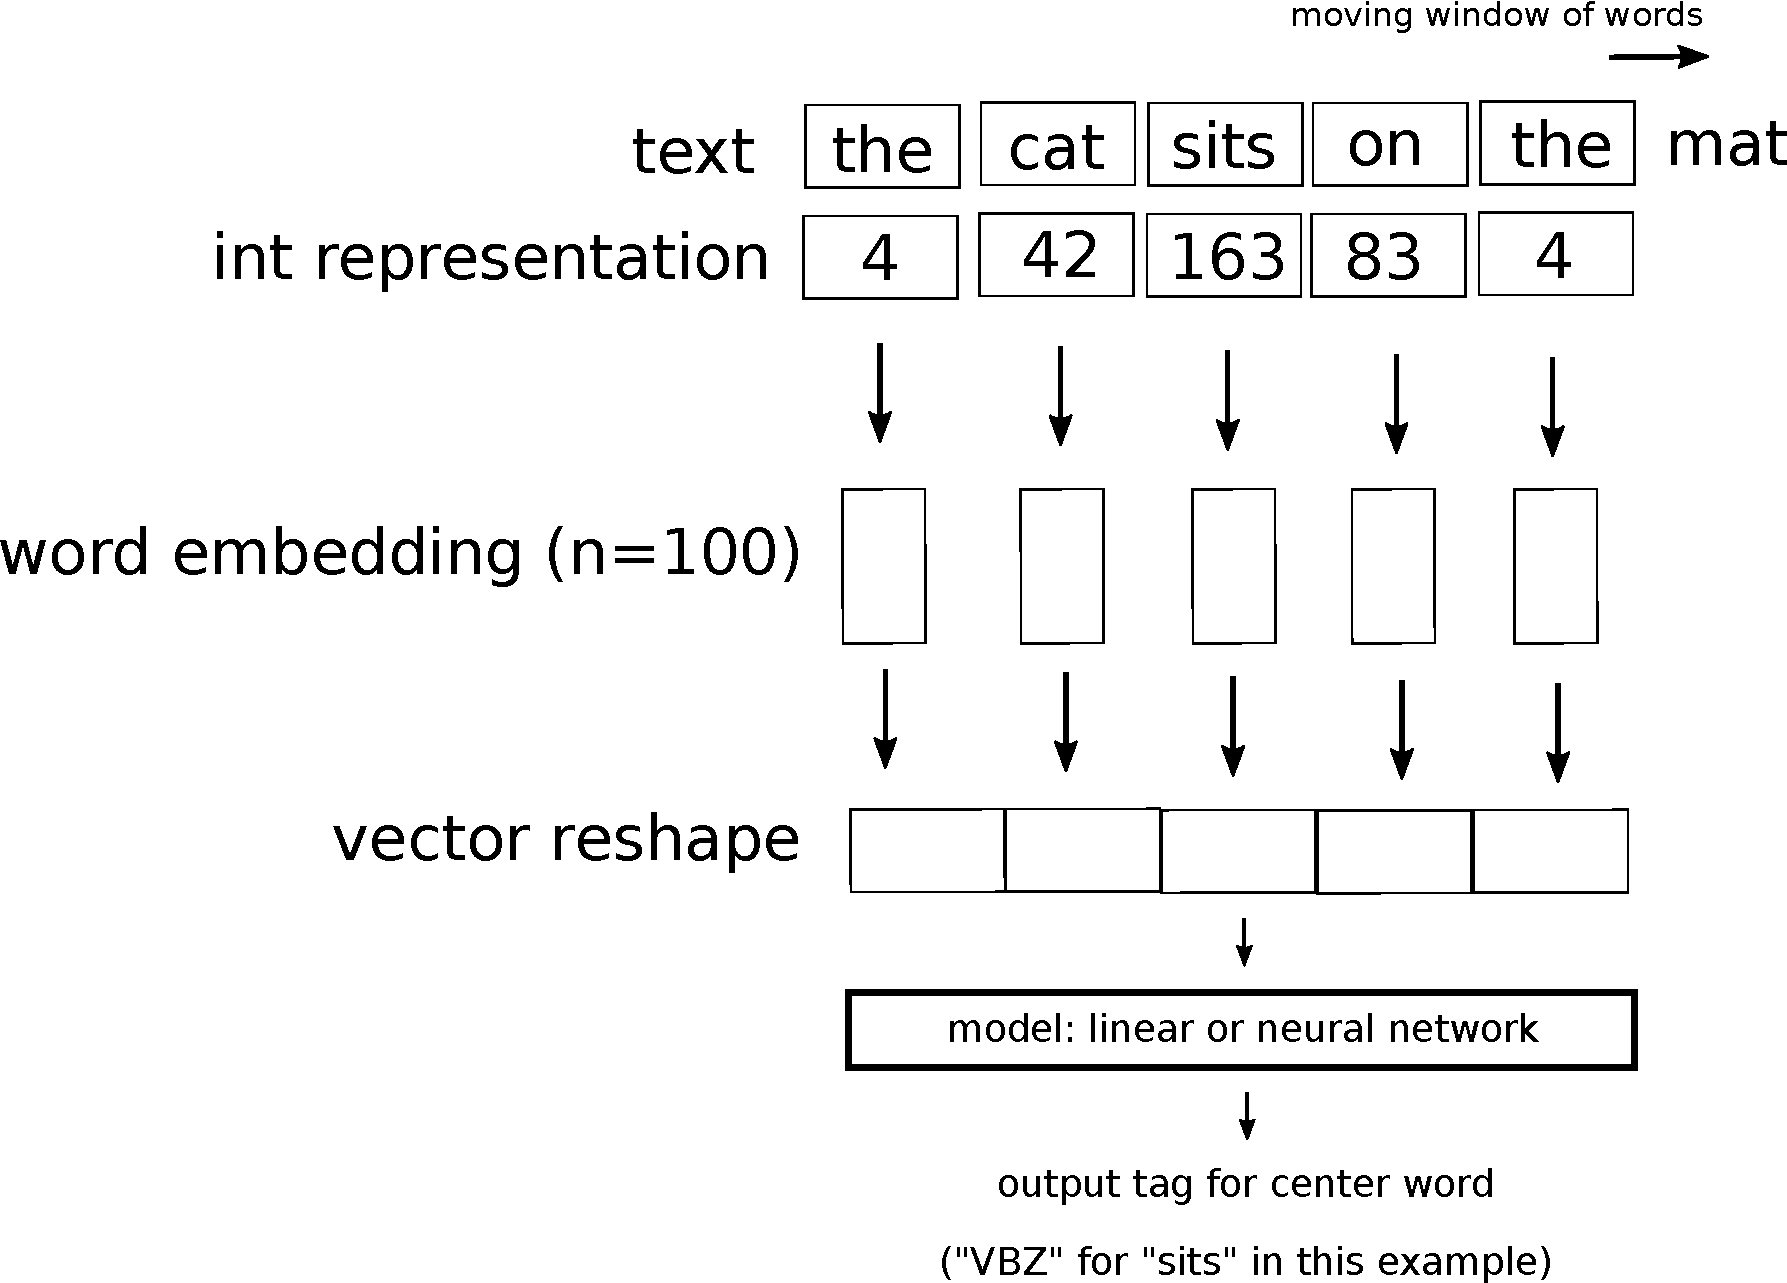
\includegraphics[height=30ex]{postagger1.pdf}
\end{frame}

\section{Embedding layer}

\begin{frame}[fragile]
  \frametitle{Sparse encoding of one-hot values}

  [``A'', ``short'', ``example''] → [3011, 291, 14]
  \vspace{2ex}

  \lstinline{sklearn.preprocessing.LabelEncoder()} does this

  \pause
  .fit → extract the vocabulary from data and assign Integers\\
  .transform → apply the mapping

  \pause
  \textcolor{reduhh}{Does not handle unseen values}

  \pause
  \vspace{2ex}
  Can be used directly to compute the (softmax) cross entropy loss
\begin{lstlisting}
  tf.nn.sparse_softmax_cross_entropy_with_logits(
      labels=y_train, logits=pred)
\end{lstlisting}

  \lstinline{y_train} is expected to be an array of Integers

   
\end{frame}



%\begin{frame}
%  \frametitle{Cross entropy loss}
%
%  \begin{itemize}
% \item Generalization of the logistic loss to multiple classes:
%  \end{itemize}
%  
%  $\xi(t,y) = - \sum_{i=1}^{n} \left[ t_i log(y_i) + (1-t_i)log(1-y_i) \right]$  
%  
%\end{frame}


\begin{frame}
  \frametitle{Embeddings}

  Embedding layer:\\$emb: V → \mathbb{R}^d$

  \vspace{2ex}
  Embedding matrix:\\$\left| V \right| \times d$ matrix
  
\end{frame}


 \begin{frame}[fragile]
  \frametitle{Embedding matrix}
  The embeddings matrix is a variable that we want to optimize:
  \begin{lstlisting}
embeddings = tf.Variable(
tf.random_uniform([vocabulary_size,
embedding_size], -1.0, 1.0))
\end{lstlisting}    
\end{frame}


 \begin{frame}[fragile]
  \frametitle{Embedding lookup}
  
  \begin{footnotesize}
 \begin{lstlisting}
embed = tf.nn.embedding_lookup(embeddings, train_inputs)
\end{lstlisting}
\end{footnotesize}    

e.g. If your list of sentences is: $\big[[0, 1], [0, 3]\big]$ (sentence 1 is $[0, 1]$, sentence 2 is $[0, 3]$, the function will compute a tensor of embeddings, which will be of shape $(2, 2, \text{embedding\_size})$ and will look like:
\\
$$[[\text{embedding0, embedding1}], [\text{embedding0, embedding3}]]$$

\end{frame}


\begin{frame}
  \frametitle{Flatten a sequence of inputs}

    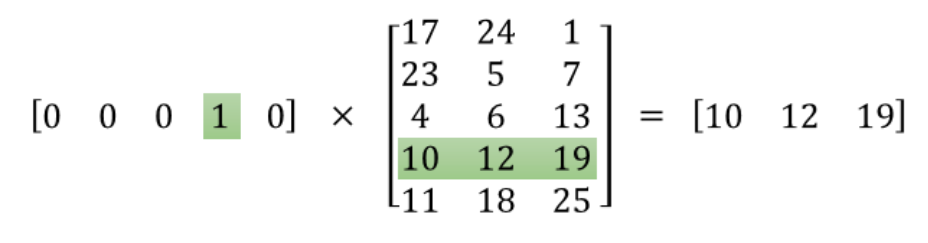
\includegraphics[height=15ex]{sparse_lookup.png}
    
    \begin{itemize}
    	\item tf.nn.embedding\_lookup does a sparse matrix multiplication for the lookup
    \end{itemize}
\end{frame}


\begin{frame}
  \frametitle{Flatten a sequence of inputs}

  \begin{displaymath}
    \begin{pmatrix} x_{1,1} & \hdots & x_{1,embedding\_size}\\\vdots && \vdots\\x_{n,1} & \hdots & x_{n,embedding\_size}\end{pmatrix}
  \end{displaymath}

  →

  \begin{displaymath}
    \begin{pmatrix} x_{1,1} & \hdots & x_{1,embedding\_size} & \hdots & x_{n,1} & \hdots & x_{n,embedding\_size}\end{pmatrix}
  \end{displaymath}

  \pause\vspace{2ex}

  Tensorflow has \lstinline{tf.reshape} to do that
  
\end{frame}


\begin{frame}[fragile]
  \frametitle{Flatten a sequence of embeddings}


  Input: tensor of rank 3 ([examples, seq\textunderscore len, embedding\textunderscore size])\\
  Output: tensor of rank 2 ([examples, embedding\textunderscore size*seq\textunderscore len])
  
 
  \begin{footnotesize}
\begin{lstlisting}
# tensor 't' is [[[0.344, 1.12], [-0.12, 0.11]],
#                [[0.344, 1.12], [3.1, -1.78]]]
# tensor 't' has shape [2, 2, 2]
# (2 examples of length 2 with embeddings of dim 2)
reshape(t, [2, 4]) ==> [[0.344, 1.12, -0.12, 0.11],
                        [0.344, 1.12, 3.1, -1.78]]
\end{lstlisting}
  \end{footnotesize}

  \vspace{1ex} \pause
  Special value -1:
  If one component of shape is the special value -1, the size of that dimension
  is computed so that the total size remains constant. [\ldots] At most one component of shape can be -1.
  {\tiny\url{https://www.tensorflow.org/api_docs/python/tf/reshape}}
  
\end{frame}

\section{Multinomial logistic regression}

\begin{frame}
  \frametitle{Softmax function}
$\sigma(\bf{z})_j = \frac{e^{z_j}}{\sum_{k=1}^K e^{z_k}}$ for ''j'' = 1, …, ''K''.

  \begin{itemize}
 	 \item Transforms the vector z, so that all values add up to one
 	 \item Can be used as a probability distribution over outputs (=classes)
 	 \item Commonly used in neural networks as output function for classification tasks
  \end{itemize}
\end{frame}


\begin{frame}
  \frametitle{Cross entropy}
  
%  \begin{itemize}
%  \item Softmax is a generalization of the Sigmoid function for $n$ categories.
%  \item squashes the values in a vector into values between $0$ and $1$, the sum
%    of the values is $1$
%  \end{itemize}
%
%  \pause

  Cross-entropy (for $C$ classes):

  \begin{displaymath}
    - \sum_{i=1}^n\sum_{c=1}^C y_{ic}\log{p_{ic}}
  \end{displaymath}

$p_{i} p_{i}$ is the true label

  Note: For two classes this is binary-crossentropy

%  In tensorflow use: \lstinline{tf.nn.softmax_cross_entropy_with_logits}

\end{frame}

\begin{frame}[fragile]
  \frametitle{Softmax and cross entropy in Tensorflow}

\begin{lstlisting}
  tf.nn.softmax_cross_entropy_with_logits(
  labels=y_train, logits=pred)
\end{lstlisting}

vs.

\begin{lstlisting}
  tf.nn.sparse_softmax_cross_entropy_with_logits(
  labels=y_train, logits=pred)
\end{lstlisting}

  \begin{itemize}
 \item Difference is how y\_train is given:
 \item e.g. $\big[[0 0 0 1 0], [0 0 0 0 1]\big]$ vs. $[3,4]$ or $[0,0,1,0]$ vs. $[2]$
  \end{itemize}

\end{frame}

\begin{frame}
  \frametitle{Hands on: A simple POS tagger}

  A POS tagger (Brown corpus)

  \begin{itemize}
  \item use an embedding layer
  \item predict the POS tag given the embeddings of the target word and $n$
    context words
  \end{itemize}
  
\end{frame}

\begin{frame}
  \frametitle{Getting the predicted class}

  \begin{itemize}
  \item Getting the class index:\\
    \lstinline{tf.argmax} returns the index of the largest value in a tensor\pause
  \item Getting the class names:\\
    Use \lstinline{.inverse_transform} of a LabelEncoder to transform sparse
    one-hot encodings back to non-numeric labels
  \end{itemize}
  
\end{frame}

\section{Deep Feed-Forward Networks}

\begin{frame}
  \frametitle{A feed-forward DNN}
  \begin{center}
    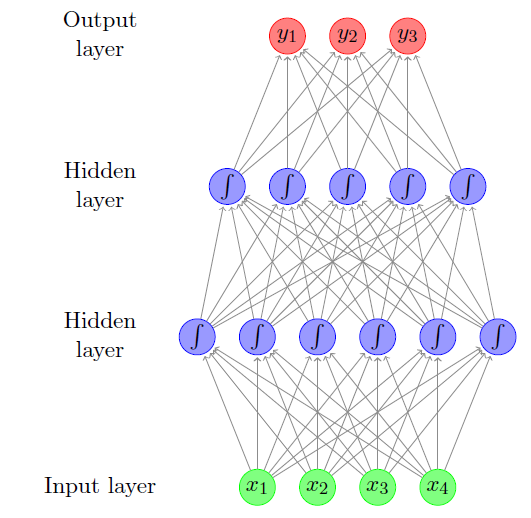
\includegraphics[height=30ex]{03-goldberg-ffn.png}
  \end{center}
  % Goldberg: A Primer on Neural Network Models for Natural Language Processing
\end{frame}

\begin{frame}[fragile]
  \frametitle{Multiple layers}

  First approach: just add layers
  \begin{footnotesize}
\begin{lstlisting}
last_dim = input_dim
for dim in [100, 100]:
    hidden = tf.Variable(tf.random_uniform(
        [last_dim, dim], -0.1, 0.1, dtype=tf.float32))
    b = tf.Variable(tf.random_uniform(
        [dim], -0.1, 0.1, dtype=tf.float32))
    x = tf.add(tf.matmul(x, hidden), b)
    last_dim = dim
\end{lstlisting}
  \end{footnotesize}
  \pause 
  Won't add anything to the models capacity:\\
  as each layer is just a linear function this is just composing linear
  functions -- the result is a linear function

\end{frame}

\begin{frame}[fragile]
  \frametitle{Adding non-linearities}
  Different choices: Sigmoid, tanh, ReLU (Rectified Linear Unit)
  
  \begin{footnotesize}
\begin{lstlisting}
last_dim = input_dim
for dim in [100, 100]:
    hidden = tf.Variable(tf.random_uniform(
        [last_dim, dim], -0.1, 0.1, dtype=tf.float32))
    b = tf.Variable(tf.random_uniform(
        [dim], -0.1, 0.1, dtype=tf.float32))
    x = tf.add(tf.matmul(x, hidden), b)
    x = tf.nn.relu(x)
    last_dim = dim

\end{lstlisting}
  \end{footnotesize}
\end{frame}

\begin{frame}
  \frametitle{Non-linearities}
  %https://www.quora.com/Why-do-non-zero-mean-activations-induce-a-bias-shift-for-units-in-the-next-layer-and-why-is-that-bad
 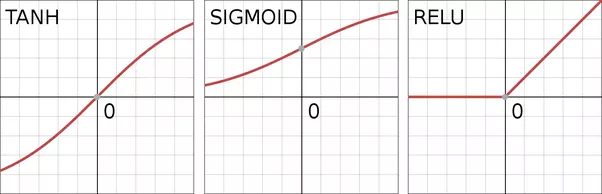
\includegraphics[width=\textwidth]{nonlinear.png} 

 \lstinline{tf.tanh} \hfill \lstinline{tf.sigmoid} \hfill \lstinline{tf.nn.relu}
\end{frame}

\begin{frame}
  \frametitle{MLP with one hidden layer}

  One hidden layer is enough to create a universal approximator.\\\pause

  However:\\
  Neural networks with more layers have been shown to learn functions better.
  
\end{frame}


\begin{frame}[fragile]
  \frametitle{Example}
  
  \begin{footnotesize}
\begin{lstlisting}
last_dim = input_dim
for dim in [100, 100]:
    ### add hidden layers as before

## define the output layer
out_w = tf.Variable(tf.random_uniform(
      [last_dim, out_dim], -0.1, 0.1,
      dtype=tf.float32))
b = tf.Variable(tf.random_uniform(
    [out_dim], -0.1, 0.1, dtype=tf.float32))
out = tf.add(tf.matmul(x, out_w), b)
\end{lstlisting}
  \end{footnotesize}
\end{frame}


\begin{frame}
  \frametitle{Hands on 1}

  Add hidden layers to the POS tagger.
  
\end{frame}

\begin{frame}[fragile]
  \frametitle{Dropout}

\begin{itemize}
\item   Srivastava, Nitish, et al. "Dropout: a simple way to prevent neural networks from overfitting." Journal of machine learning research 15.1 (2014): 1929-1958.
\end{itemize}
  
  In Tensorflow:
  \begin{verbatim}
   tf.nn.dropout( x,  keep_prob, noise_shape=None,  
   									seed=None,   name=None)
  \end{verbatim}
  
\end{frame}

\begin{frame}[fragile]
  \frametitle{Hands on 2}

  Extend POS tagger with a train a test set, measure accuracy. (Hint: \verb#sklearn.metrics.accuracy_score#)
  Add dropout to the POS tagger and compare train and validation loss+accuracy.
  
\end{frame}

\begin{frame}[fragile]
 
 \frametitle{Tensorboard}
  \begin{itemize}
		\item Visualize loss, embeddings and much more in your browser
		\item You need to add a few lines of code to tell Tensorboard what to log
		\item Make sure train\_summary\_dir is a new directory for every new experiment!
	\end{itemize}
			
	\begin{tiny}
\begin{lstlisting}
 loss_summary = tf.summary.scalar('loss', loss) 
 train_summary_op = tf.summary.merge_all()
 summary_writer = tf.summary.FileWriter(train_summary_dir, sess.graph)
\end{lstlisting}   
\end{tiny}    
	
\end{frame}

\begin{frame}[fragile]
 
 \frametitle{Tensorboard}
  \begin{itemize}
		\item You need to regularly call the train\_summary\_op in training
		\item Not as often as the training step, because it will otherwise slowdown your training if you have more complex summaries
	\end{itemize}
			
\begin{tiny}
\begin{lstlisting}
if current_step % 100==0 and current_step != 0:
	summary_str = sess.run(train_summary_op, feed_dict=feed_dict)
	summary_writer.add_summary(summary_str, current_step)
	summary_writer.flush()
\end{lstlisting}   
\end{tiny}    
	
\end{frame}

\begin{frame}[fragile]
 
 \frametitle{Tensorboard}
  \begin{itemize}
		\item Some useful statistics on tensors (e.g. neural network weights):
	\end{itemize}
\begin{tiny}
\begin{lstlisting}
with tf.name_scope('x1'):
        tf.summary.scalar('mean', mean)
        with tf.name_scope('stddev'):
            stddev = tf.sqrt(tf.reduce_mean(tf.square(var - mean)))
        tf.summary.scalar('stddev', stddev)
        tf.summary.scalar('max', tf.reduce_max(var))
        tf.summary.scalar('min', tf.reduce_min(var))
        tf.summary.histogram('histogram', var)
\end{lstlisting}   
\end{tiny}  
\end{frame}


\begin{frame}[fragile]
 \frametitle{Tensorboard - running it}
 \begin{tiny}
 \begin{lstlisting}
tensorboard  --logdir=w2v_summaries_1499773534
--host=127.0.0.1
or
python3 -m tensorboard.main  --logdir=w2v_summaries_1499773534
--host=127.0.0.1
\end{lstlisting}   
\end{tiny}
 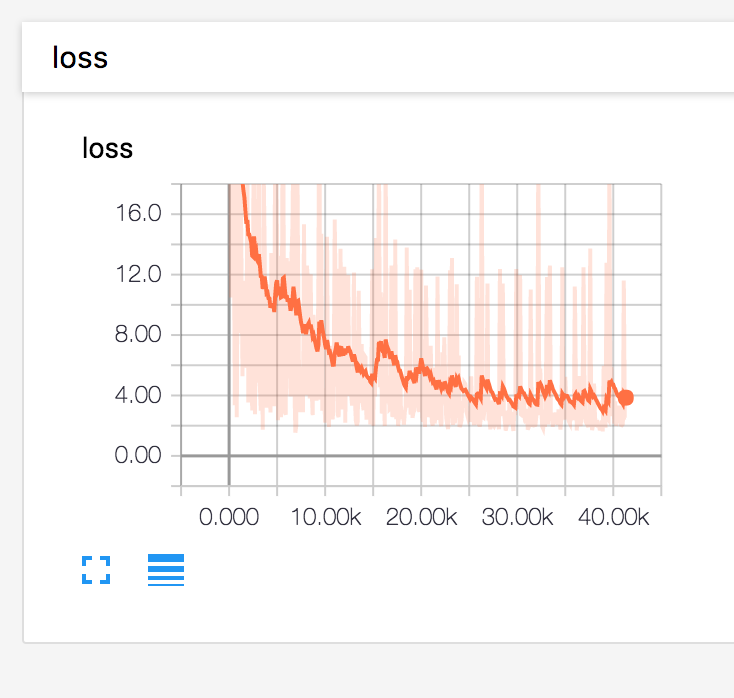
\includegraphics[width=0.4\textwidth]{04_loss}
\end{frame}


\begin{frame}[fragile]
 \frametitle{Tensorboard - embeddings}
   \begin{itemize}
		\item Possible to nicely visualize embeddigs, see \url{https://www.tensorflow.org/get_started/embedding_viz}
		\item Also checkout \url{http://projector.tensorflow.org/}, live demo of pretrained embeddings
		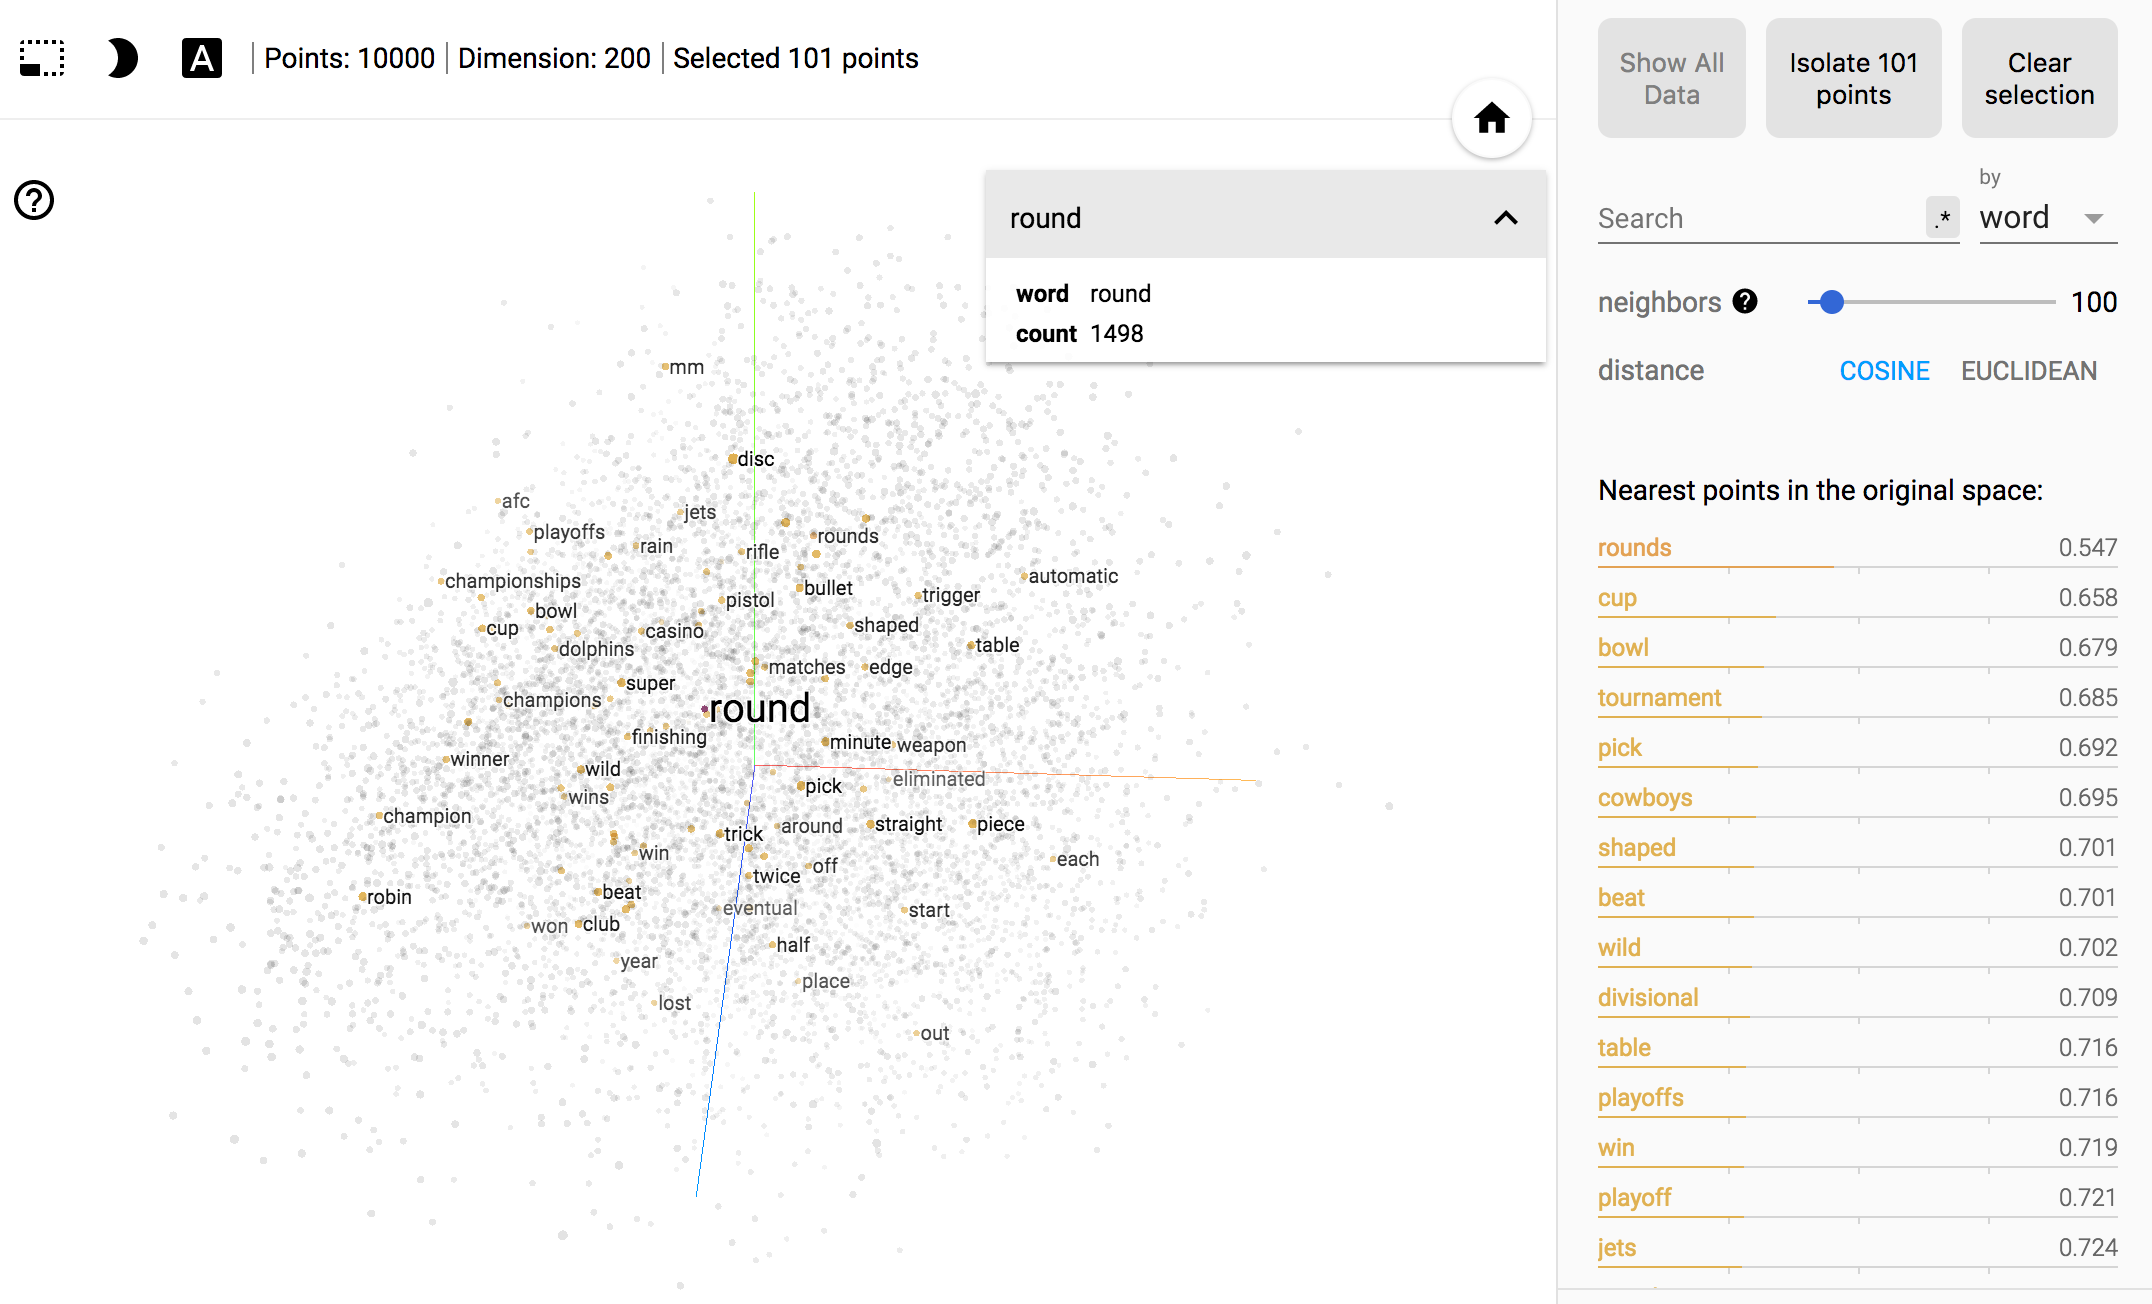
\includegraphics[width=0.5\textwidth]{04_embed_viz.png}
	\end{itemize}
\end{frame}



\end{document}


%%% Local Variables:
%%% mode: latex
%%% TeX-engine: luatex
%%% End:
